\section{Why shared resources?}


%%%%%%%---- BEGIN ----  ----%%%%%%
\begin{frame}
  \frametitle{A typical research project}

  \begin{columns}[T]

    \begin{column}{.4\textwidth}
      \begin{overlayarea}{\textwidth}{\textheight}
        \only<1>{\hspace{0.05\hsize}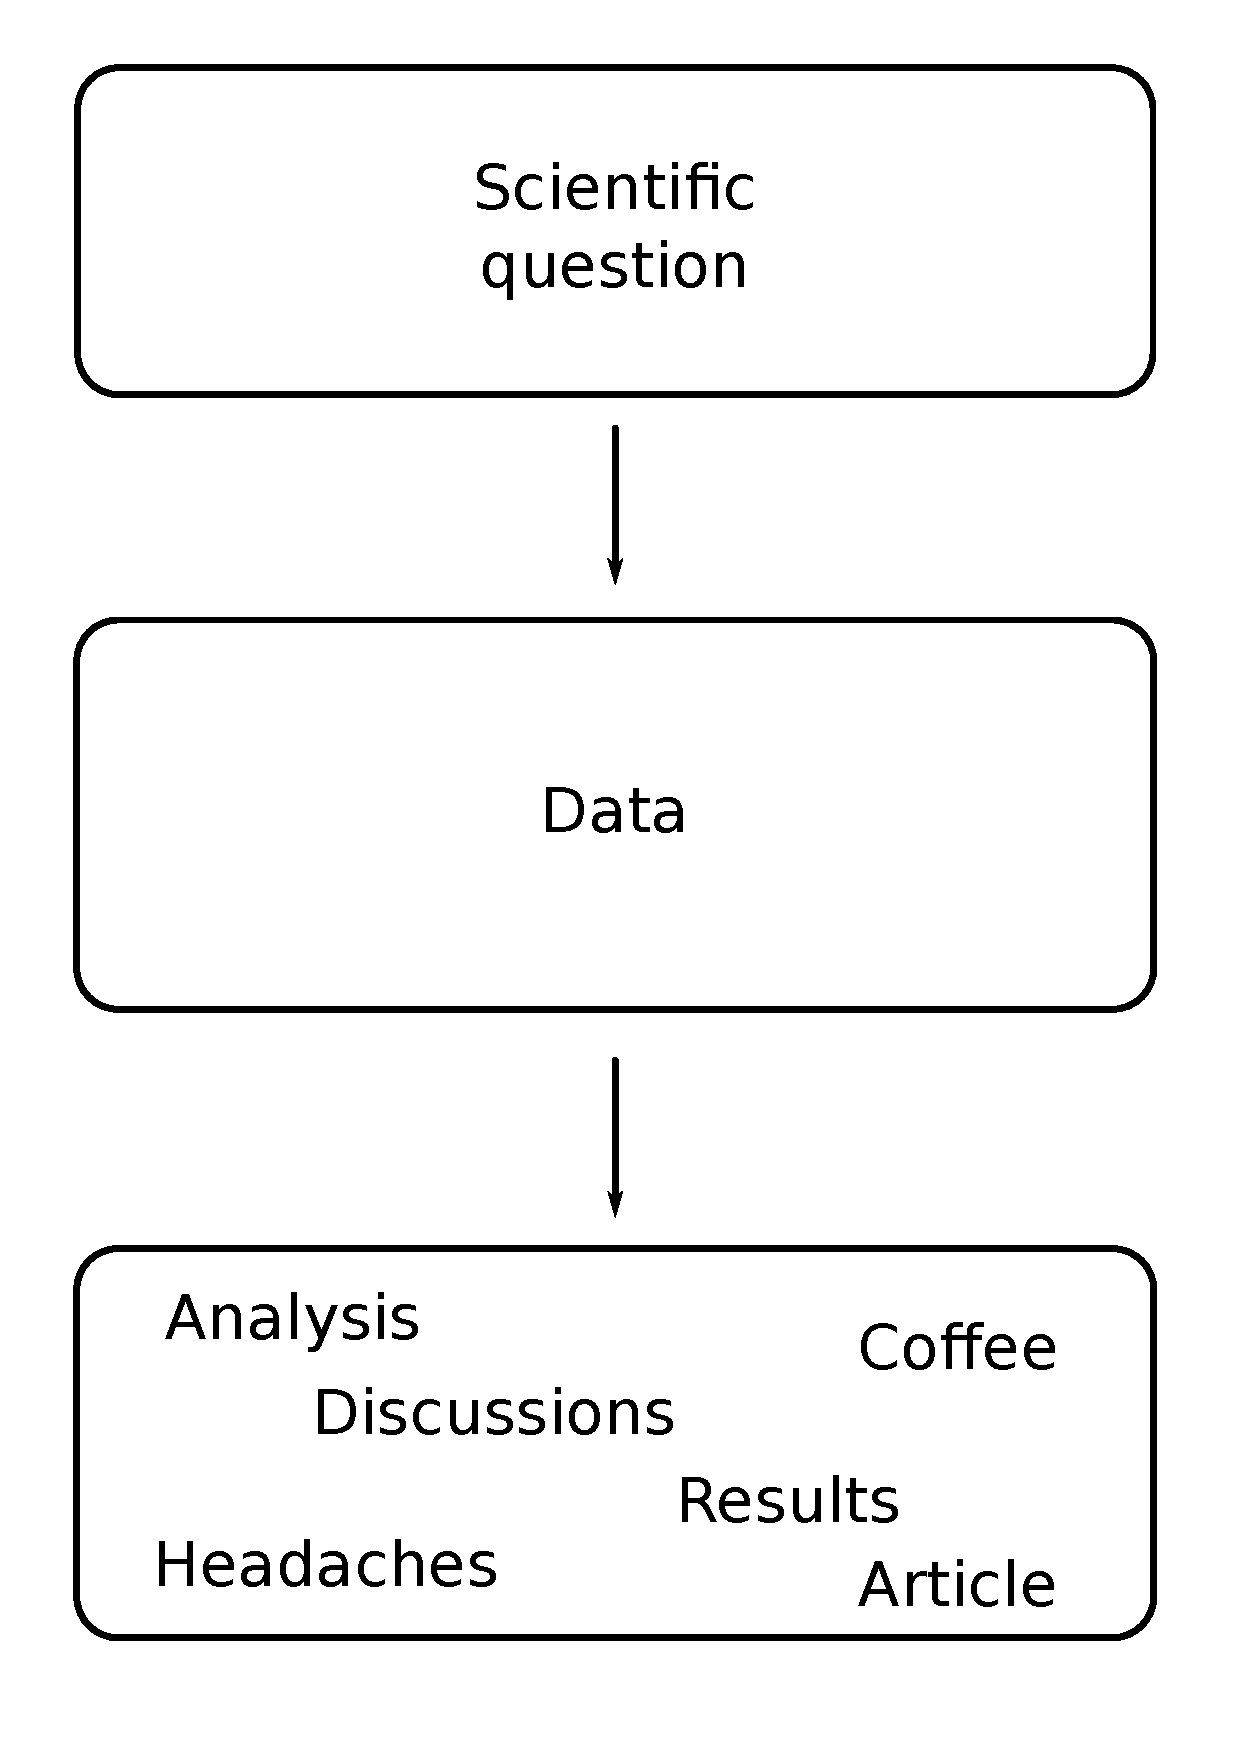
\includegraphics[width=0.9\hsize]{sci_project_1}}
        \only<2>{\hspace{0.05\hsize}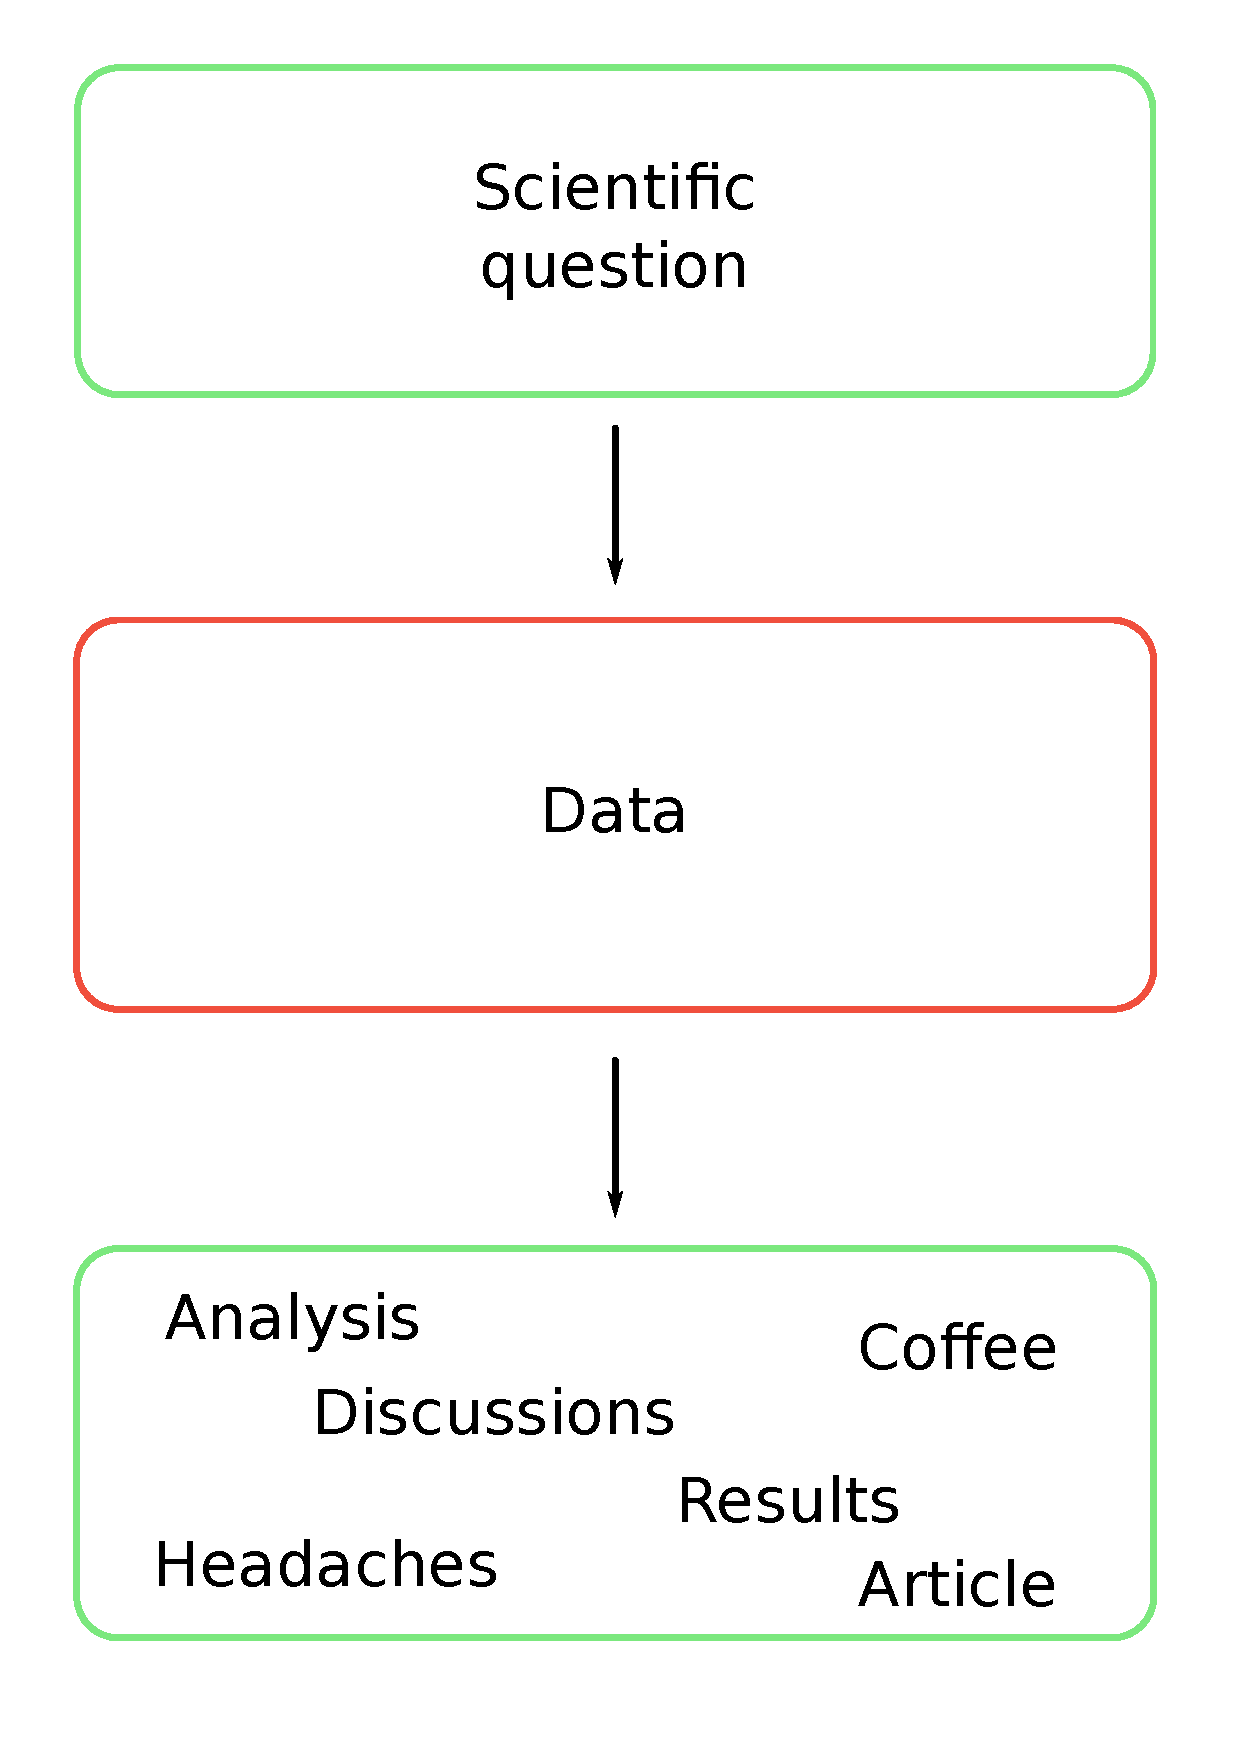
\includegraphics[width=0.9\hsize]{sci_project_2}}
      \end{overlayarea}
    \end{column}


    \begin{column}{.6\textwidth}
      \begin{overlayarea}{\textwidth}{\textheight}
        \begin{onlyenv}<2>

          \vspace{1em}
          \textbf{Repetitive (and tedious) tasks!}\\
          \vspace{1em}
          \begin{itemize}[<.->]
            \item \emph{Planning and conduction of observations}
              \begin{itemize}[<.->]
                \item[$\circ$] Observations already exist?
                \item[$\circ$] Target/sample available? visible?
              \end{itemize}

            \vspace{0.5em}
            \item \emph{Gathering ancillary data for the analysis}
              \begin{itemize}[<.->]
                \item[$\circ$] Complementary information \src{diameter, fall/find, ...}
                \item[$\circ$] Context for research \src{another population}
              \end{itemize}

            \vspace{0.5em}
            \item \emph{Repetitive low-level analysis}
              \begin{itemize}[<.->]
                \item[$\circ$] Spectral classification
                \item[$\circ$] Cross-matches \& merges
              \end{itemize}

          \end{itemize}
        \end{onlyenv}
      \end{overlayarea}
    \end{column}
  
  \end{columns}

\end{frame}
%%%%%%%----  END  ----  ----%%%%%%



%%%%%%%---- BEGIN ----  ----%%%%%%
\begin{frame}
  \frametitle{Shared resources save community time}

  \begin{itemize}[<.->]
    \item \emph{Tedious task? Share the load!}
      \begin{itemize}[<.->]
        \item[$\circ$] Many agencies have the mission to support the community
        \item[$\circ$] Target/sample available? visible?
      \end{itemize}
  
    \vspace{0.5em}
    \item \emph{Gathering ancillary data for the analysis}
      \begin{itemize}[<.->]
        \item[$\circ$] Complementary information \src{diameter, fall/find, ...}
        \item[$\circ$] Context for research \src{another population}
      \end{itemize}
  
    \vspace{0.5em}
    \item \emph{Validation}
      \begin{itemize}[<.->]
        \item[$\circ$] Spectral classification
        \item[$\circ$] Cross-matches \& merges
      \end{itemize}

  \end{itemize}
  
\end{frame}
%%%%%%%----  END  ----  ----%%%%%%




